\section{Prototypes and Results}

\subsection{Disclaimer}
\subsubsection{Completed Prototypes}
Originally, the following three prototypes were planned.
\begin{itemize}
    \item volumetric rendering
    \item procedural noise generation
    \item ray marching
\end{itemize}
While researching the topic and experimenting with some dummy shaders, it came clear that "\gls{volumetricrendering}" and "\gls{raymarching}" are interchangeable in this matter.
Therefore, only two kinds of prototyping have been developed. This change is explained in detail in \autoref{section:projectmanagement}

\subsubsection{Dimensions}
All of the following documented procedures and algorithms were prototyped and implemented in 3D, but for the matter of explanation, it is described and visualized in 2D.

\subsubsection{Unity Variables}
The following sections will list code snippets, in which all variables prefixed with an underscore are shader variables exposed to the Unity Editor. This way, they can be changed externally while running the shader code, allowing for convenient debugging.
They are from here on out referred to as \textit{\gls{parameters}}.

\clearpage
\subsection{First Draft}
The first drafts of prototypes created during this project all revolve around volumetric rendering. 
Instead of using a \gls{sdf}, a noise function was used. The primary issue was to get the cube transparent where the noise function would return a number close to 0.0 and to color it where the number would be close to 1.0.
The approach for solving this issue is done by sampling the cloud's density instead.

\subsubsection{Density sampling}
Like in \gls{volumetricrendering}, for each pixel fragment, a ray is cast from the fragment into the cube, along the view direction for that fragment.
Usually, the algorithm can stop for a given ray if the \gls{sdf} returns a small enough distance, meaning the ray has hit a surface of the volume. However, it is different in the case with clouds, where the volume is \textit{\gls{translucent}} at most points.
\\
To account for that, the ray does not stop until the end of the container cube is reached. It samples the density $N$ times along its path and returns the sum of those samples, giving an approximate qualifier for how dark this fragment should be.

\begin{figure}[H]
    \centering
    \begin{tikzpicture}[scale=1.2]
        \tikzset{edge/.style = {-{Latex[length=3mm]},shorten >= -4pt}}
        \tikzset{shortedge/.style = {-{Latex[length=3mm]},shorten <=-4pt,shorten >= -4pt}}
        \tikzset{icon/.style = {font=\Large}}

        % icons
        \node[icon,rotate=35,anchor=west] (cam) at (0, 0) {\faVideoCamera};

        % clouds
        \node[cloud, cloud puffs=15.7, minimum width=5cm, minimum height=3.5cm, align=center, draw] (cloud) at (4.5, 3.5) {};
        \node[cloud, cloud puffs=15.7, minimum width=2cm, minimum height=1.5cm, align=center, draw] (cloud) at (5.0, 1.1) {};
        \node[cloud, cloud puffs=15.7, minimum width=3cm, minimum height=2.0cm, align=center, draw] (cloud) at (0.2, 3.5) {};
        \node[cloud, cloud puffs=15.7, minimum width=1.5cm,minimum height= 1cm, align=center, draw] (cloud) at (1.75, 0.9) {};

        % outer point
        \node (pOut) at (7, 5.25) {};
        \draw[red, edge] (cam) -- (pOut) node[midway,above,sloped,xshift=-3cm] {};

        % cloud points
        \node[red] (p1) at (1.5, 1.125) {\textbullet};
        \node (p2) at (2.5, 1.875) {\textopenbullet};
        \node[red] (p3) at (3.5, 2.625) {\textbullet};
        \node[red] (p4) at (4.5, 3.375) {\textbullet};
        \node[red] (p5) at (5.5, 4.125) {\textbullet};

        \node[red, yshift=0.4cm] at (p1) {$p_1$};
        \node[red, yshift=0.4cm] at (p2) {$p_2$};
        \node[red, yshift=0.4cm] at (p3) {$p_3$};
        \node[red, yshift=0.4cm] at (p4) {$p_4$};
        \node[red, yshift=0.4cm] at (p5) {$p_5$};


        \end{tikzpicture}
    \captionof{figure}{Density sampler ray with $N = 5$.}
    \label{img:tikz:prototypes:densitysampling}
\end{figure}

\noindent
Understandably, the bigger clouds in \autoref{img:tikz:prototypes:densitysampling} represent higher return values of the noise function, meaning denser areas.
For the displayed ray, the values for points $p_1, p_3, p_4$ and $p_5$ are accumulated and used as a qualifier to color the fragment. In this case, a rather dark tone would be used.
\\
It is notable that $N$ has a linear impact on the performance, so it should be chosen carefully.

\begin{figure}[H]
    \centering
    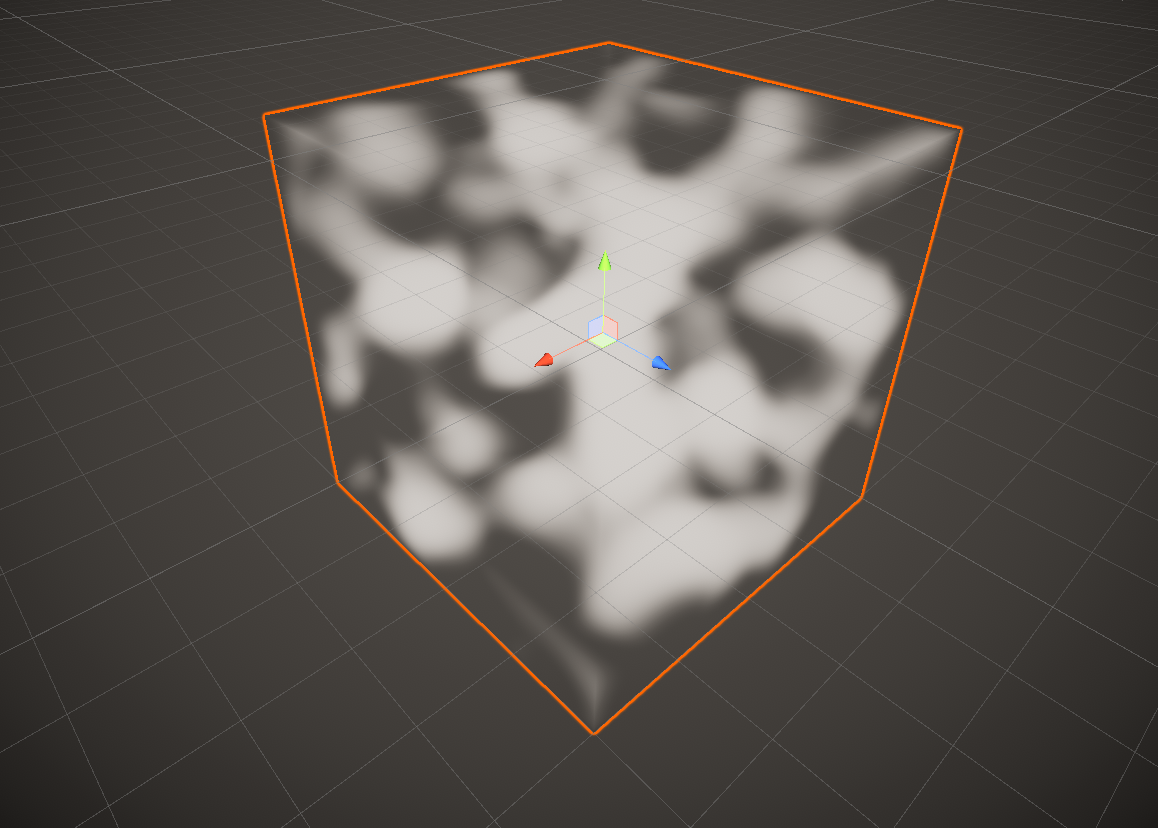
\includegraphics[width=\linewidth]{unity captures/prototype1.PNG}
    \captionof{figure}{Prototype: Rendered image of sampled density based on 3D Perlin noise.}
    \label{img:captures:prototype1}
\end{figure}

\noindent
With this first try, a Perlin noise function was sampled. The returned value had to be normalized in a range of $[0, 1]$ in order to for it to be used as alpha value of the color.

\subsubsection{Normalizing Density}
This is where the exponential function $exp(x) = e^{-x}$ comes in, which (when clamped from 0 to 1) converts very low values to 1.0 and higher values will converge towards 0.0.

\begin{figure}[H]
    \centering
    \begin{minipage}{0.47\linewidth}
        \begin{tikzpicture}
            \begin{axis}[
                axis lines=center,
                samples=50,
                xmin=-0.5,
                xmax=4.5,
                ymin=-0.2,
                ymax=1.2,
                xlabel={$x$},
                ylabel={$y$},
                xlabel style={below right},
                ylabel style={above left},
                height=4cm,
                width=8cm,
                ytick={0,1},
                xtick={0,1,2,3,4},
                ]
    
                \addplot[red] plot (\x, { exp(-\x)) });
            \end{axis}
        \end{tikzpicture}
        \captionof{figure}{Exponential function $exp(x) = e^{-x}$.}
        \label{img:math:exp}
    \end{minipage}        
    \hfill
    \begin{minipage}{0.47\linewidth}
        \begin{tikzpicture}
            \begin{axis}[
                axis lines=center,
                samples=50,
                xmin=-0.5,
                xmax=4.5,
                ymin=-0.2,
                ymax=1.2,
                xlabel={$x$},
                ylabel={$y$},
                xlabel style={below right},
                ylabel style={above left},
                height=4cm,
                width=8cm,
                ytick={0,1},
                xtick={0,1,2,3,4},
                ]
    
                \addplot[red] plot (\x, { 1 - exp(-\x)) });
            \end{axis}
        \end{tikzpicture}
        \captionof{figure}{Inverted exponential function $exp'(x) = 1 - e^{-x}$.}
        \label{img:math:exp1}       
    \end{minipage}
\end{figure}

\noindent
When inverting $exp(x)$, the function $exp'(x)$ returns a value that can be directly used for the transparency of the cloud. The denser it gets, the more opaque it will be.

\clearpage
\subsection{Improving Noise}
After further experimenting with the noise sampling function, the idea arose to combine Perlin and Voronoi noise, which hopefully would create a more distinguished, random pattern.
The final sampling function simply multiplies both noise values at a given point \lstinline[language=HLSL]{position}. 

\begin{lstlisting}[language=HLSL, numbers=left, caption=Implementation of a density sampling function., label=lst:shader:prototype:sampledensity]
float sampleDensity(float3 position) {
  float3 vpos = position * _VoronoiScale + _VoronoiOffset;
  float3 ppos = position * _PerlinScale + _PerlinOffset;
  float vd = getColorVoronoi(vpos, _VoronoiOctaves, _VoronoiPersistance));
  float pd = getColorPerlin(ppos, _PerlinOctaves, _PerlinPersistance));
  
  vd = max(0, vd - _VoronoiDensityThreshold) * _VoronoiDensityMultiplier;
  pd = max(0, pd - _PerlinDensityThreshold) * _PerlinDensityMultiplier;
  
  // fix boost density by factor 2
  float density = vd * pd * 2.0;
  return density;
}
\end{lstlisting}

\noindent
By adjusting some of the \gls{parameters} and increasing the octaves of both noises, a more patchy and cloudy look can be achieved at the cost of performance.

\begin{figure}[H]
    \centering
    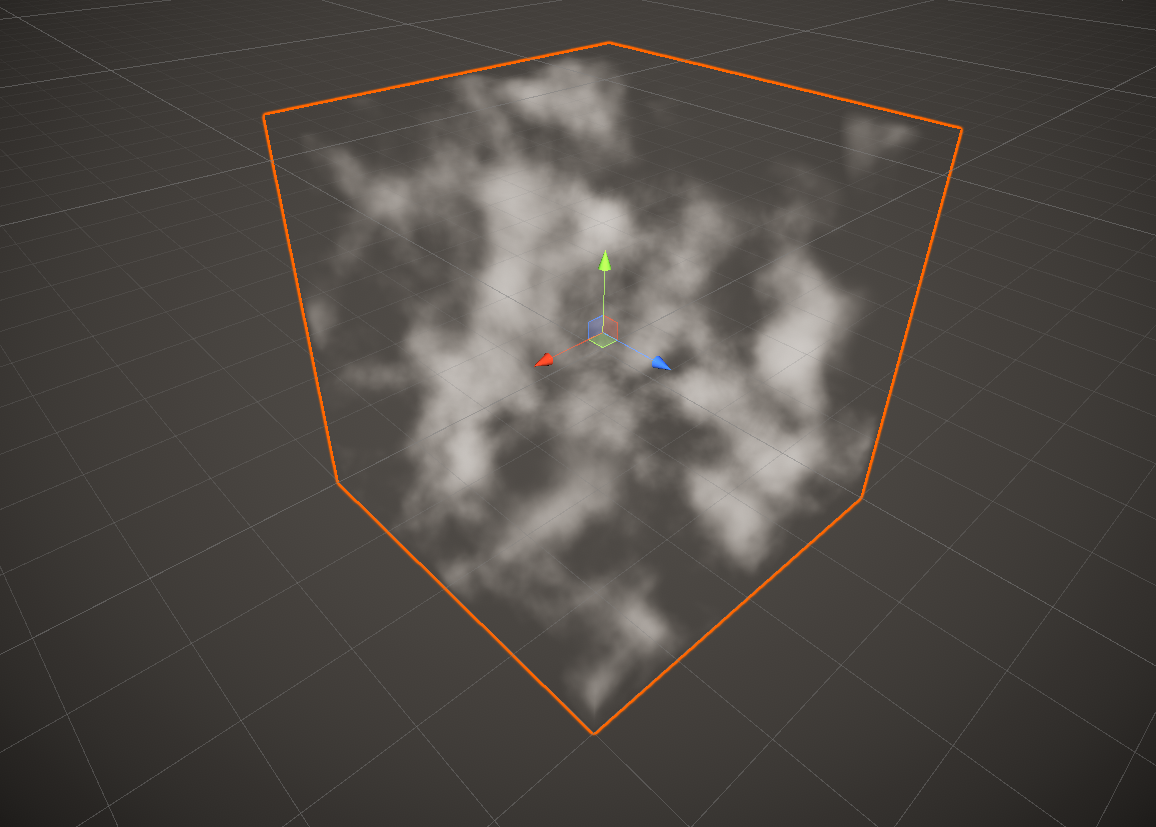
\includegraphics[width=\linewidth]{unity captures/prototype2.PNG}
    \captionof{figure}{Prototype: Rendered image of sampled density based on mixed noises.}
    \label{img:captures:prototype2}
\end{figure}

\clearpage
\subsection{Light Transmittance and Light Scattering}
One of the more prominent lighting features of clouds is its translucency. It describes how light bounces and scatters inside the matter, then exits at a different point. This is called \textit{\gls{sss}} (SSS).
It results in illuminated areas where the clouds are thinner. In nature, \gls{sss} is a very complex and computationally demanding process. For computer graphics however, it is often either simplified or substituted with some other algorithm that produces a similar outcome at lower performance cost.

\subsubsection{Sunlight Forwarding}
When approaching the implementation of \gls{sss} and directional lighting, it seemed most reasonable to start with the sun being visible behind the clouds, or at least shining through them.
This implies finding a way to illuminate clouds that cover the sun. In the context of this project, it is called \textit{\gls{sunlighttransmittance}} or \textit{\gls{sunlightforwarding}}, since it is not a variant of SSS but rather an approximation.
\\
After some consideration and brainstorming, the following method was chosen to solve the issue:

\begin{figure}[H]
    \centering
    \begin{tikzpicture}[scale=1.2]
        \tikzset{edge/.style = {-{Latex[length=3mm]},shorten >= -4pt}}
        \tikzset{shortedge/.style = {-{Latex[length=3mm]},shorten <=-4pt,shorten >= -4pt}}
        \tikzset{line/.style = {shorten >=-4pt}}
        \tikzset{icon/.style = {font=\Large}}

        % icons
        \node[icon,rotate=35,anchor=west] (cam) at (0, 0) {\faVideoCamera};
        \node[icon] (light) at (8, 6) {\faLightbulbO};
        \node at (8, 6.5) {light source};

        % clouds
        \node (cloud) at (4.0, 5.2) {};
        \node[cloud, cloud puffs=15.7, cloud, minimum width=3.5cm, minimum height=2.2cm, align=center, draw] (cloud) at (cloud) {};

        % screen space
        \draw (1,1) -- (5,1) -- (5,4);

        % rays
        \node[red] (p1) at (3, 2.25) {\ding{53}};
        \node[red] (st1) at ($(p1) + (0.5, -0.2)$) {$st_2$};

        \node[cyan,mark=x] (c1) at (2.4, 2.4) {\ding{53}};
        \node[cyan] (st2) at ($(c1) + (-0.5, 0.2)$) {$st_1$};

        \node (p2) at (5, 3.75) {};
        \node (c2) at (4, 4) {};
        \node[cyan] (c3) at (5.1, 5.1) {\textbullet};

        \draw[red, line] (cam) -- (p1);
        \draw[red, line, loosely dashed] (p1) -- (p2);
        \draw[red, edge, loosely dashed] (p2) -- (light);
        
        \draw[cyan, line] (cam) -- (c1);
        \draw[cyan, line, loosely dashed] (c1) -- (c2);
        \draw[cyan, edge, loosely dashed] (c2) -- (c3);

        % rest of screen space
        \draw (5,4) -- (1,4) node[anchor=south west] {screen space} -- (1,1);

        \end{tikzpicture}
    \captionof{figure}{Sunlight transmittance sampling (1).}
    \label{img:tikz:prototypes:sunlight}
\end{figure}

\noindent
When ray casting, both the fragment's and the light source's screen-space position is calculated. Those are two-dimensional coordinates relative to the screen that the camera renders to.
Now if the distance $d = \norm{\overrightarrow{st_1 st_2}} < t$, with $t$ being some threshold, a portion of the sun's color is added to the fragment's color, relative to how small $d$ is.

\begin{figure}[H]
    \centering
    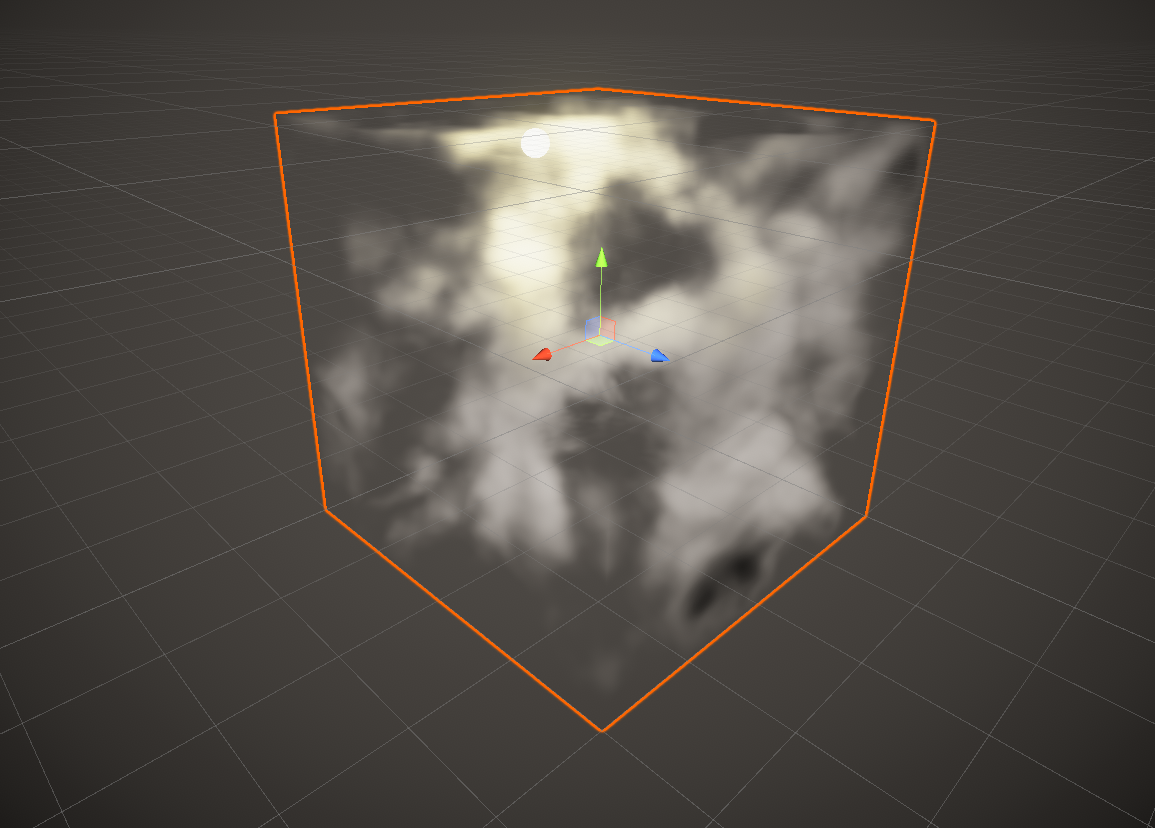
\includegraphics[width=\linewidth]{unity captures/prototype4.PNG}
    \captionof{figure}{Prototype: Rendered image of sunlight transmittance.}
    \label{img:captures:prototype3}
\end{figure}

\noindent
Behind the cube in \autoref{img:captures:prototype3} is a sphere object placed, representing the sun. The sunlight is indeed shining through the clouds, but there are still some minor flaws with the implementation.
For example, some clouds are completely illuminated, making them too bright where the cloud would be too dense for the light to pass through.
\emptyline
The following code snippet shows the implementation of the sunlight transmittance mechanism. The \lstinline[language=HLSL]{density} variable is the one evaluated in \autoref{lst:shader:prototype:sampledensity}.

\begin{lstlisting}[language=HLSL, caption=Implementation of a sunlight transmittance mechanism., label=lst:shader:prototype:sampledensity]
float cloudDensity = exp(-density);

float projectedSunDistance = length(
  worldToScreenPos(_SunPosition) - worldToScreenPos(worldPosition));

float sunTransmittance = 1 - pow(
  smoothstep(0.01, _SunLightScattering,projectedSunDist), _SunLightStrength);

fixed3 sunColor = sunTransmittance * _LightColor0.xyz * cloudDensity;
\end{lstlisting}

\noindent
Like in other prototype code listings, there are some \gls{parameters} to play with. The sunlight strength or the sunlight range (in screen space) can both be adjusted, for example.
\\
The idea of multiplying by \lstinline[language=HLSL]{cloudDensity} on line 9 was to fix the previously described flaw of clouds being too bright. 

\clearpage
\subsubsection{Directional light}
Another challenging part during prototyping was directional light reflections on surfaces facing the sun. Usually in \gls{raymarching}, a \gls{surfacenormal} estimation is done using the gradient.
This works well if there is only one point of interest (like a surface hit), but as already mentinoned before, the ray does not stop sampling points until it reaches the end of the container cube.
\\
So instead of calculating normals for each sample point, another ray is cast from the sample point towards the sun.
Along its path, the density is sampled again $L$ times in constant steps. Without an official term, this process is called \textit{\gls{lightmarching}} in this project.

\begin{figure}[H]
    \centering
    \begin{tikzpicture}[scale=1]
        \tikzset{edge/.style = {-{Latex[length=3mm]},shorten >= -4pt}}
        \tikzset{shortedge/.style = {-{Latex[length=3mm]},shorten <=-4pt,shorten >= -4pt}}
        \tikzset{lightedge1/.style = {-{Latex[length=3mm]},shorten <=-4pt,shorten >= 0.8cm}}
        \tikzset{lightedge2/.style = {-{Latex[length=3mm]},shorten <=-4pt,shorten >= 0.85cm}}
        \tikzset{lightedge3/.style = {-{Latex[length=3mm]},shorten <=-4pt,shorten >= 0.90cm}}
        \tikzset{icon/.style = {font=\Large}}

        % icons
        \node[icon,rotate=35,anchor=west] (cam) at (1, 0.75) {\faVideoCamera};
        \node[icon] (light) at (1, 6) {\faLightbulbO};
        \node at (1, 6.5) {light source};

        % clouds
        \node (cloud) at (4.5, 3.5) {};
        \node[cloud, cloud puffs=15.7, cloud ignores aspect, minimum width=5cm, minimum height=3.5cm, align=center, draw] (cloud) at (cloud) {};

        % outer point
        \node (pOut) at (7, 5.25) {};

        % rays
        \draw[red, edge] (cam) -- (pOut) node[midway,above,sloped,xshift=-3cm] {};
        
        % cloud points
        \node[red] (p1) at (3.5, 2.625) {\textbullet};
        \node[red] (p2) at (4.5, 3.375) {\textbullet};
        \node[red] (p3) at (5.5, 4.125) {\textbullet};
        \node[red] (p4) at (4.5, 3.375) {\textbullet};
        \node[red] (p5) at (5.5, 4.125) {\textbullet};

        % light march rays
        \draw[cyan, lightedge1] (p1) -- (light) node[midway,above] {};
        \draw[cyan, lightedge2] (p2) -- (light) node[midway,above] {};
        \draw[cyan, lightedge3] (p3) -- (light) node[midway,above,yshift=0.5cm] {lightmarch rays};

        % light sample points
        \node[cyan] (l1) at (3.25, 2.95) {\textbullet};
        \node[cyan] (l2) at (4.15, 3.625) {\textbullet};
        \node[cyan] (l3) at (5.0, 4.325) {\textbullet};
        
        \node[cyan] (l5) at (3.0, 3.3) {\textbullet};
        \node[cyan] (l6) at (3.75, 3.95) {\textbullet};
        \node[cyan] (l7) at (4.5, 4.55) {\textbullet};
        
        \node[cyan] (l8) at (2.75, 3.65) {\textbullet};
        \node[cyan] (l9) at (3.35, 4.22) {\textbullet};
        \node[cyan] (l10) at (3.95, 4.775) {\textbullet};

        \end{tikzpicture}
    \captionof{figure}{Directional sunlight transmittance sampling (1).}
    \label{img:tikz:prototypes:lightmarching1}
\end{figure}

\noindent
It is clearly visible that in \autoref{img:tikz:prototypes:lightmarching1}, a lot of density samples return a high value, resulting in a dark fragment color for this ray.
To simplify, there is a lot of cloud mass in front of that intersection point, so the point will not receive a lot of light.
\\
On the other hand, in \autoref{img:tikz:prototypes:lightmarching2}, only very few samples are even inside the cloud, resulting in a low value overall. This leads to a higher influence of the sun's color for that fragment, meaning it is more exposed to the sun.

\begin{figure}[H]
    \centering
    \begin{tikzpicture}[scale=1]
        \tikzset{edge/.style = {-{Latex[length=3mm]},shorten >= -4pt}}
        \tikzset{shortedge/.style = {-{Latex[length=3mm]},shorten <=-4pt,shorten >= -4pt}}
        \tikzset{lightedge1/.style = {-{Latex[length=3mm]},shorten <=-4pt,shorten >= 0.8cm}}
        \tikzset{lightedge2/.style = {-{Latex[length=3mm]},shorten <=-4pt,shorten >= 0.85cm}}
        \tikzset{lightedge3/.style = {-{Latex[length=3mm]},shorten <=-4pt,shorten >= 0.90cm}}
        \tikzset{icon/.style = {font=\Large}}

        % icons
        \node[icon,rotate=35,anchor=west] (cam) at (1, 0.75) {\faVideoCamera};
        \node[icon] (light) at (1, 6) {\faLightbulbO};
        \node at (1, 6.5) {light source};

        % clouds
        \node (cloud) at (5.7, 2.7) {};
        \node[cloud, cloud puffs=15.7, cloud ignores aspect, minimum width=5cm, minimum height=3.5cm, align=center, draw] (cloud) at (cloud) {};

        % outer point
        \node (pOut) at (7, 5.25) {};

        % rays
        \draw[red, edge] (cam) -- (pOut) node[midway,above,sloped,xshift=-3cm] {};
        
        % cloud points
        \node[red] (p1) at (3.5, 2.625) {\textbullet};
        \node[red] (p2) at (4.5, 3.375) {\textbullet};
        \node[red] (p3) at (5.5, 4.125) {\textbullet};
        \node[red] (p4) at (4.5, 3.375) {\textbullet};
        \node[red] (p5) at (5.5, 4.125) {\textbullet};

        % light march rays
        \draw[cyan, lightedge1] (p1) -- (light) node[midway,above] {};
        \draw[cyan, lightedge2] (p2) -- (light) node[midway,above] {};
        \draw[cyan, lightedge3] (p3) -- (light) node[midway,above,yshift=0.5cm] {lightmarch rays};

        % light sample points
        \node (l1) at (3.25, 2.95) {\textopenbullet};
        \node[cyan] (l2) at (4.15, 3.625) {\textbullet};
        \node (l3) at (5.0, 4.325) {\textopenbullet};
        
        \node (l5) at (3.0, 3.3) {\textopenbullet};
        \node (l6) at (3.75, 3.95) {\textopenbullet};
        \node (l7) at (4.5, 4.55) {\textopenbullet};
        
        \node (l8) at (2.75, 3.65) {\textopenbullet};
        \node (l9) at (3.35, 4.22) {\textopenbullet};
        \node (l10) at (3.95, 4.775) {\textopenbullet};

        \end{tikzpicture}
    \captionof{figure}{Directional sunlight transmittance sampling (2).}
    \label{img:tikz:prototypes:lightmarching2}
\end{figure}

\clearpage
\noindent
The implementation for \gls{lightmarching} is rather straight-forward, given the concept of \gls{raymarching} is already known.

\begin{lstlisting}[language=HLSL, caption=Implementation of lightmarching., label=lst:shader:prototype:lightmarching]
float lightmarch(float3 position, float3 direction) {
    float3 p = position;

    float lightTransmittance = 0;
    for (int j = 0; j < _MaxLightSteps; j++)
    {
        p += direction * _LightStepSize;
        lightTransmittance += sampleDensity(p);
    }

    return lightTransmittance;
}
\end{lstlisting}

\noindent
The method is called during \gls{raymarching} and the original function is modified like so:
\begin{lstlisting}[language=HLSL,caption=Implementation of raymarching with lightmarching., label=lst:shader:prototype:raylightmarching]
float2 raymarch(float3 position, float3 direction)
{
    float3 sunDirection = normalize(_SunPosition - position);
    float lightStepSize = insideBoxDist / _MaxLightSamples;
    float lightTransmittance = 0;

    [...ray marching...]
    
    for (int j = 0; j < _MaxLightSamples; j++)
    {
        position += direction * lightStepSize;
        lightTransmittance += lightmarch(position, sunDirection);
    }

    return float2(density, lightTransmittance);
}
\end{lstlisting}

\noindent
Now, two values are returned instead of just one. Both are later normalized with either $exp(x)$ or $exp'(x)$.

\begin{figure}[H]
    \centering
    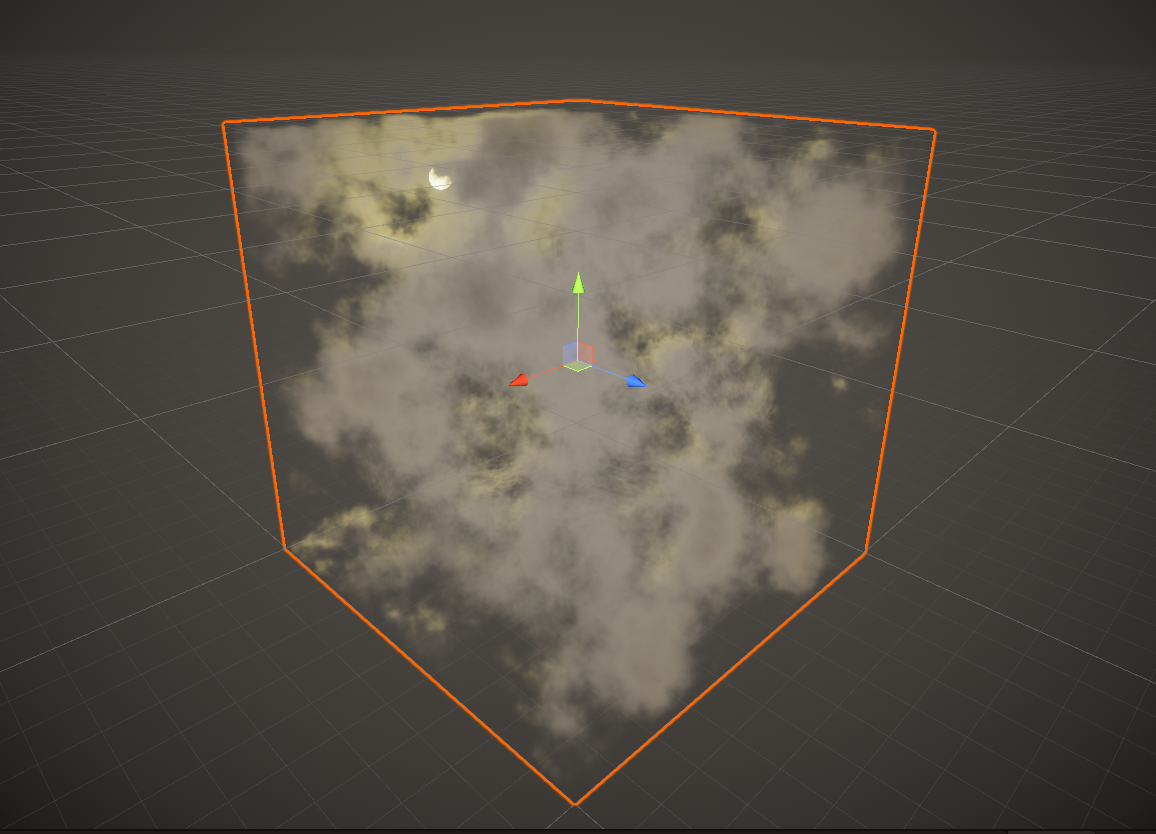
\includegraphics[width=\linewidth]{unity captures/prototype5.PNG}
    \captionof{figure}{Prototype: Rendered image of directional sunlight implemented with \gls{lightmarching}.}
    \label{img:captures:prototype3}
\end{figure}

\clearpage
\subsection{Final Prototype}
All put together and after quite some effort and experimenting, the rendered scene looks quite convincing.

\begin{figure}[H]
    \centering
    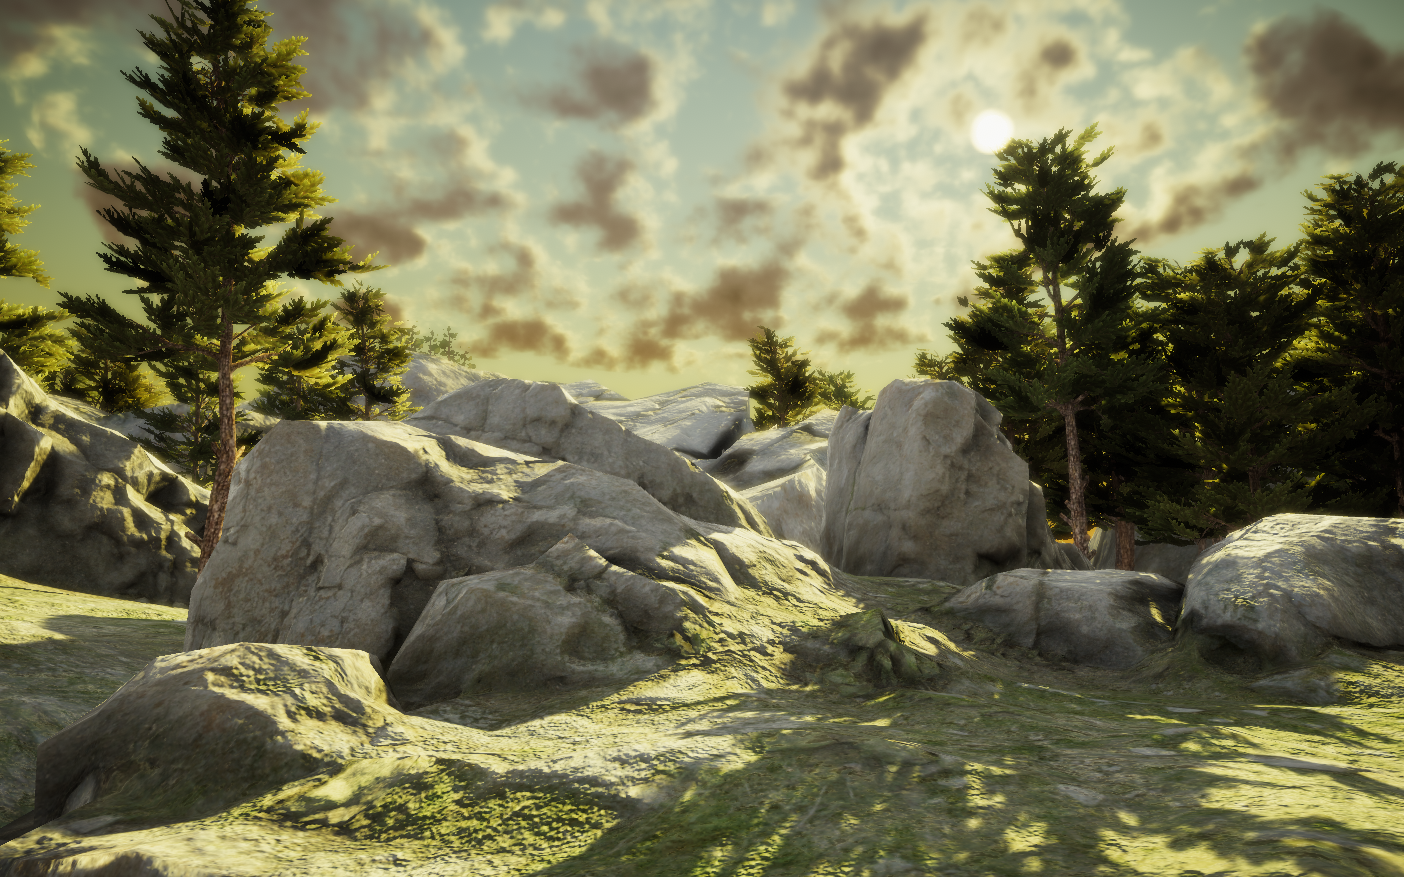
\includegraphics[width=\linewidth]{unity captures/final shot prototype 2.PNG}
    \captionof{figure}{Prototype: Rendered image of the final prototype.}
    \label{img:captures:prototype_final}
\end{figure}